58. Получить числа 5 и 16 можно только как $5:1=7$ и $8\times2=16.$ Тогда из остальных цифр нужно выбрать два, дающих в сумме 11 это могут быть только 7 и 4. Три оставшихся цифры как раз образуют пример на вычитание.
\begin{center}
\begin{figure}[ht!]
\center{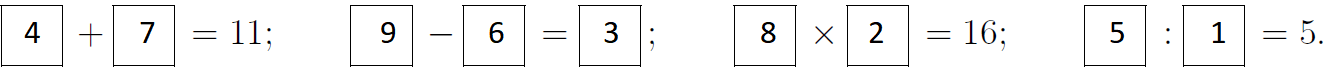
\includegraphics[scale=0.35]{111s.png}}
\end{figure}
\end{center}
